\chapter{Pin Control Attack analysis}
\label{chap:analysis}

Before describing Pin Control Attack, a deeper analysis of the architecture of the target system is needed.
Note that, although this paper is focused on PLCs, the architecture described in the next section is still valid for almost any embedded system.
After having a proper knowledge of the underlying architecture, we can go deep into the description of the attack.
We consider the idea behind I/O attack, showing how it is able to evade the currently available detection mechanisms.
Next, we go further extending the applicability to a real Programmable Logic Controller, describing its architecture in more detail.
Based on our architecture analysis and our tests, we can finally demonstrate that the attack is actually viable on real PLCs, even on a higher abstraction level.


\section{Embedded architecture}

As briefly reported into \chap \ref{chap:intro}, PLCs use I/O interfaces to communicate with sensors and actuators, and in general with any external device.
Digging into their architecture, we know that PLCs are usually based on a so called System on Chip (SoC).
A SoC is basically an integrated circuit made of a microprocessor, a memory block and a set of peripheral controllers all enclosed together in the same chip substrate.
Thus, the SoC technology provides fully capable computers having both very small size and low power-consumption.
A SoC usually comes with a set of I/O interfaces, called \emph{pins}. I/O pins are soldered to an external board to facilitate interconnection with external modules.
An example of such a system is the Raspberry Pi board shown in \myfig{\ref{fig:raspberry}}, based on a Broadcom System on Chip.
\begin{figure}[h]
\centerline{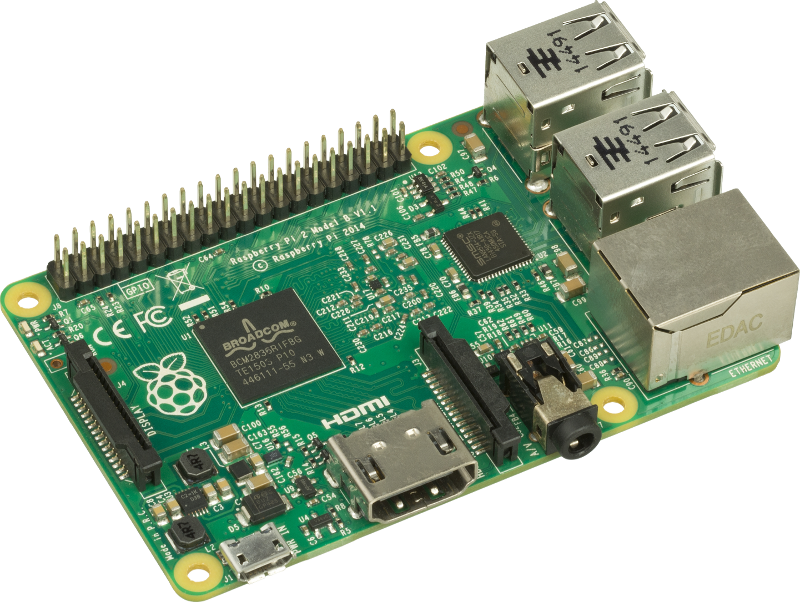
\includegraphics[width=0.56\textwidth]{res/raspberry}}
\caption{Raspberry Pi \cite{raspberry} with Broadcom System on Chip \label{fig:raspberry}}
\end{figure}
Actually almost all of the embedded systems use a SoC with similar boards, each one with its own size and configuration.

In order to accommodate different potential implementations, each pin (or group of pins) of a SoC may have multiple configuration and operating modes,
depending on the board they are attached to. The configuration of the pins is managed by the pin controller, a particular subsystem of any SoC.
Through the pin controller, the system can configure the operating mode of the pins, such as their input or output mode.
The features of a pin controller can be grouped into two main categories:
\begin{itemize}
	\item Pin configuration: allows the system to change some electrical properties of the pins (see \sec \ref{sec:iopins});
	\item Pin multiplexing: each pin of the SoC may have many usage usages, also known as \emph{alternate functions}, depending on what is needed by the external board.
		The pin multiplexing feature enables the system to specify which type of function is needed on each pin.
\end{itemize}
As the I/O attack is a very low-level attack, it is necessary to dig further into the electrical world to know how these I/O interfaces work.


\subsection{I/O pins}
\label{sec:iopins}

I/O interfaces of a System on Chip provides a connection between internal modules and external electronic devices.
As shown in \myfig{\ref{fig:chips}}, they are physically visible from the outside of the chip package,
usually in the form of pins \subref{fig:pins} or soldering balls \subref{fig:balls}.

\begin{figure}[h]
\centering

\begin{subfigure}{.45\textwidth}
\centering
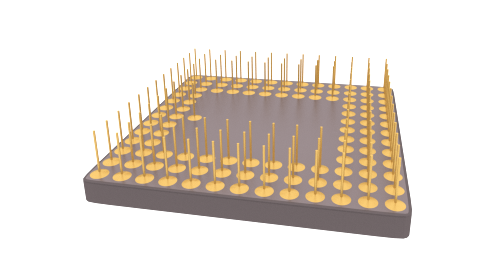
\includegraphics[width=\linewidth]{res/pins}
\caption{\label{fig:pins}}
\end{subfigure}
\begin{subfigure}{.45\textwidth}
\centering
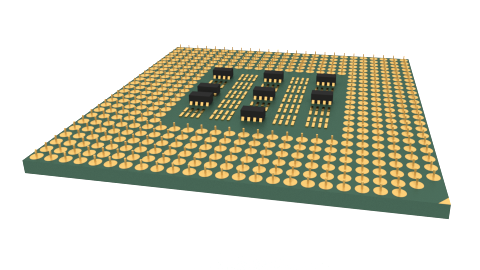
\includegraphics[width=\linewidth]{res/balls}
\caption{\label{fig:balls}}
\end{subfigure}

\caption{I/O connections packaged as \subref{fig:pins} Pin Grid Array and \subref{fig:balls} Ball Grid Array\label{fig:chips}}
\end{figure}

Internally they are connected to the silicon die through bonding wires, and are managed by a specific I/O circuit which may vary according to the specific chip.
Although there are many different implementations, almost all of the available SoCs have I/O ports with very similar functionalities.
For our purpose, we can describe them in an implementation-independent manner by using simplified generic schematics.


\subsubsection{Pin configuration}
\label{sec:pinconf}

The schematic depicted in \myfig{\ref{fig:pinconf}} helps us to discuss about the first set of features: pin configuration.
The operation mode described in this section is also known as General Purpose I/O (GPIO).

\begin{figure}[h]
\centerline{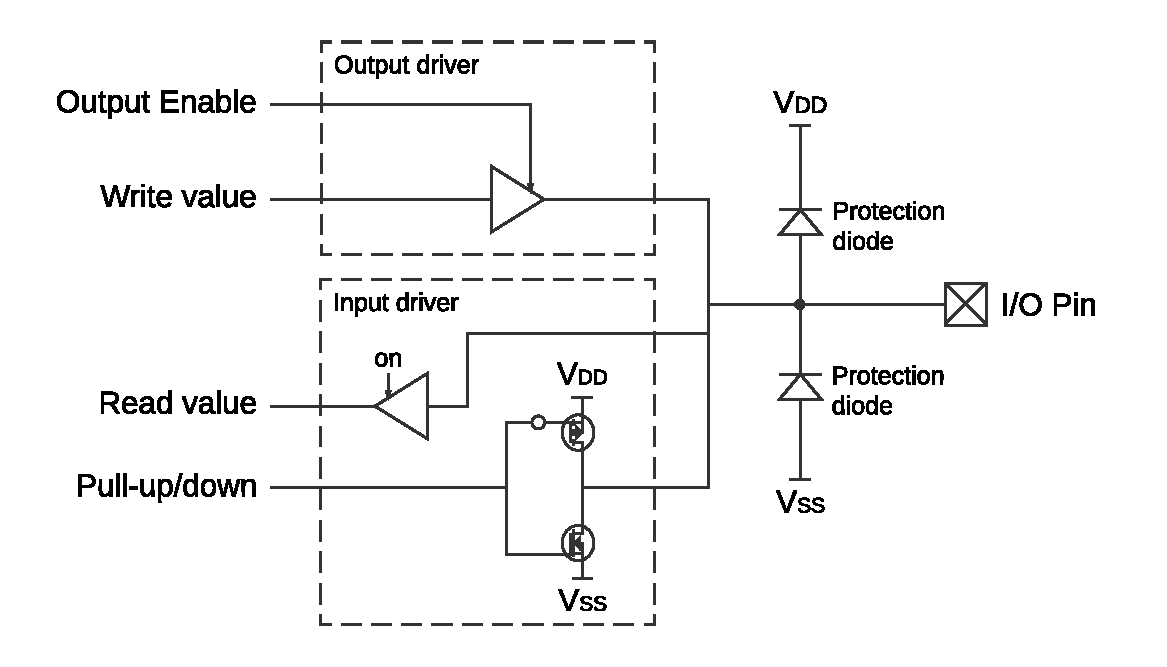
\includegraphics[width=0.8\textwidth]{res/pinconf}}
\caption{General Purpose I/O pin configuration circuit \label{fig:pinconf}}
\end{figure}

Apart from the protection diodes that serve as shield against input currents lower than $V_{SS}$ or higher than $V_{DD}$,
the circuit is divided into two different parts: one for output and one for input.
\begin{itemize}
	\item \itemname{Output driver}:
		The output module is basically a buffer controlled by an output enable signal.
		This signal controls the input or output mode of the pin. If it is high, then the pin is in output mode
		and the value coming from a write operation goes through the buffer to the actual pin.
		If it is low, the pin is in input mode and the write signal is blocked, so it is not possible to change the external value of the pin from inside anymore.
	\item \itemname{Input driver}:
		The input driver has a similar buffer to read the value, usually having hysteresis capability which is useful for filtering unstable external values.
		Since the read buffer is always active, the input value is always available, even if the pin is currently working in output mode.
		The reason for this is merely physical: even if the external value was blocked by the buffer,
		one would always get a value by reading the input signal, because a value is nothing but an interpretation of the voltage level on a wire.
		When the pin is set as input, the pull-up/pull-down network enables the user to have a ``default'' value on the pin,
		namely a defined state maintained while the pin is not actively driven from outside. This feature is useful to avoid so called ``floating'' inputs.
\end{itemize}

For Pin Control Attack, what is more interesting about the circuit in \myfig{\ref{fig:pinconf}} are the following two properties:
\begin{itemize}
	\item there is no checking about the input state, so it is possible to perform a read even when the pin is in output mode;
	\item vice versa, it is not possible to write to a pin which has been configured as output.
\end{itemize}

Furthermore, it is also possible to drive the pull-up/down network, factually disturbing the real value of the I/O pin in an unpredictable way.
In this case the effects strongly depends on the actual implementation of the circuit as well as on the capacitive load connected to the external I/O pin.


\subsubsection{Pin multiplexing}

Inside the chip an I/O pin may be connected to more than one device, which can be selected depending on the application,
that is the way of soldering or wiring the package into an electronic board.
This SoC feature is known as pin multiplexing (also ball multiplexing, pad multiplexing, alternate functions).
Even though pin multiplexing is designed for hardware configuration, in almost all modern chips it is possible to change the function at runtime.

\begin{figure}[h]
\centerline{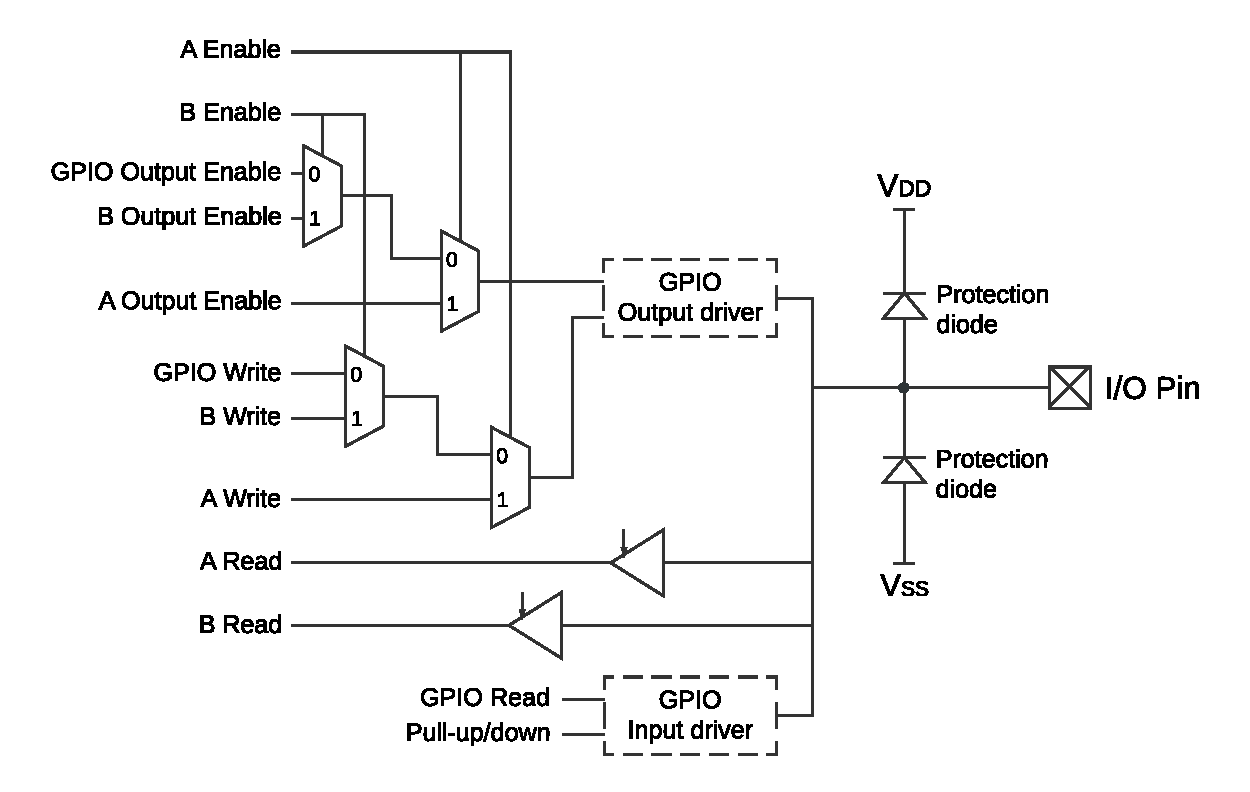
\includegraphics[width=0.8\textwidth]{res/pinmux}}
\caption{Generic I/O pin multiplexing circuit \label{fig:pinmux}}
\end{figure}

\myfig{\ref{fig:pinmux}}~ shows a possible hardware implementation of pin multiplexing.
The I/O pin in the figure is connected to two different peripherals inside the chip, namely A and B,
and it is also accessible through basic GPIO as described in \sec \ref{sec:pinconf} above.
The access to the GPIO output driver is regulated by two in cascade multiplexers for each signal of the module.
If the peripheral A is enabled, then the signals driven by A go through the multiplexers and can drive the actual value of the pin,
while GPIO and peripheral B output signals are blocked. Instead, if only peripheral B is enabled then only its signals are able to reach the I/O pin.
Note that in this last case the peripheral A should not be enabled, because A multiplexers have precedence against B ones.
Thus, the cascading of multiplexers actually implements a priority mechanism between peripherals A and B.
If neither A nor B are enabled, then no alternate function is active for the I/O pin and it could be driven by GPIO signals.
Each peripheral may also have its own dedicated input line, to get values from the I/O port in the same way as GPIO does.

For our purpose, at least two interesting properties can be inferred from pin multiplexing schematic of \myfig{\ref{fig:pinmux}}:
\begin{itemize}
	\item it is possible to block output signals from peripherals by simply changing the multiplexing configuration;
	\item the GPIO value can be read at any time, independently from the current multiplexing state of the output.
\end{itemize}


\section{Pin Control Attack}

TODO Continue with attack analysis and the rest of the chapter.
